\documentclass[conference]{IEEEtran}

\usepackage{amsmath,amssymb}
\usepackage{booktabs}
\usepackage{graphicx}
\usepackage{tabularx}
\usepackage{url}
\usepackage{xcolor}
\usepackage[hidelinks]{hyperref}

\graphicspath{{figures/pdf/}}
\newcommand{\method}{SRLinear}
\newcommand{\controller}{SRAC}
\newcommand{\hp}{HP}
\newcommand{\spot}{Spot}
\newcommand{\gpu}{GPU}

\title{Forecast Guided Reinforcement Learning for Reliable and Risk Aware Quota Control in Preemptible GPU Scheduling}

\author{\IEEEauthorblockN{Anonymous Authors}}

\begin{document}
\maketitle

\begin{abstract}
Idle capacity must be exposed to Spot jobs without delaying high priority jobs or discarding excessive completed work. Existing systems couple quota decisions to demand forecasts. Fixed control rules can become brittle under forecast error and delayed preemption cost. This paper presents Seasonal Residual Linear (SRLinear), a lightweight coherent demand forecaster and the SRLinear Risk Adaptive Controller (SRAC). SRLinear combines causal seasonal anchors, small linear residual heads, direct aggregate prediction and exact organization reconciliation. SRAC uses constrained recurrent proximal policy optimization to mix SRLinear and Contextual Linear Quota (CLQ) endpoints. Forecast uncertainty is deducted under explicit service and rollback budgets. Evaluation uses a chronological Alibaba A100 trace containing 3,456 GPUs. SRLinear obtains a mean absolute error of 154.964 with 2,052 parameters and 10.372 thousand multiply accumulate operations. It reduces mean absolute error by 5.27 percent relative to PatchTST and runs 19.39 times faster. Replacing the GFS forecast with SRLinear increases useful Spot work by 0.256 percent, reduces the Spot queue by 85.6 percent and reduces high priority violations by 66.7 percent. SRAC retains 99.9507 percent of CLQ useful work while reducing rollback loss by 2.97 percent and evictions by 4.76 percent. Its high priority violation rate remains below the 2 percent limit. These validation results apply to one homogeneous GPU type. The final August test split remains locked.
\end{abstract}

\begin{IEEEkeywords}
GPU scheduling, demand forecasting, reinforcement learning, quota control, preemption, risk constraints.
\end{IEEEkeywords}

\section{Introduction}
Modern GPU clusters are shared by high priority jobs and preemptible Spot jobs. High priority jobs require prompt gang allocation. Spot jobs use spare capacity. Their completed work can be lost when resources are reclaimed. Demand must therefore be forecast, a safe Spot quota must be set and delayed service and rollback signals must be handled.

GFS addresses this setting through organization demand forecasting, dynamic Spot quota allocation and preemption aware scheduling~\cite{gfs}. Forecast quality directly affects the capacity exposed to Spot jobs. Yet forecast error alone does not define the downstream objective. A larger quota can reduce queueing and increase useful work. It can also cause more evictions and rollback loss when high priority demand arrives. Static margins cannot express this changing tradeoff.

A second challenge is introduced by the studied A100 trace. Natural useful Spot work is close to its feasible ceiling. Local placement choices are often mapped to equivalent whole GPU nodes. Control authority is retained by quota control because the amount of Spot demand admitted before future high priority arrivals is changed. A forecast guided control problem is therefore studied instead of placement reinforcement learning.

We make three contributions.

\begin{enumerate}
\item A 2,052 parameter causal forecaster is provided by SRLinear. Multiple seasonal anchors, organization residuals, direct aggregate prediction and exact reconciliation are combined.
\item Online quota selection is formulated by SRAC as a constrained sequential decision problem. Two causal quota endpoints are mixed and forecast uncertainty is subtracted through bounded actions.
\item Forecasting, deterministic scheduling and reinforcement learning are compared in an event simulator under one chronological A100 protocol with common accounting and a fixed high priority service limit.
\end{enumerate}

Figure~\ref{fig:system} summarizes the complete control loop. Figures~\ref{fig:srlinear} and~\ref{fig:sracagent} detail the two proposed components.

\begin{figure*}[t]
\centering
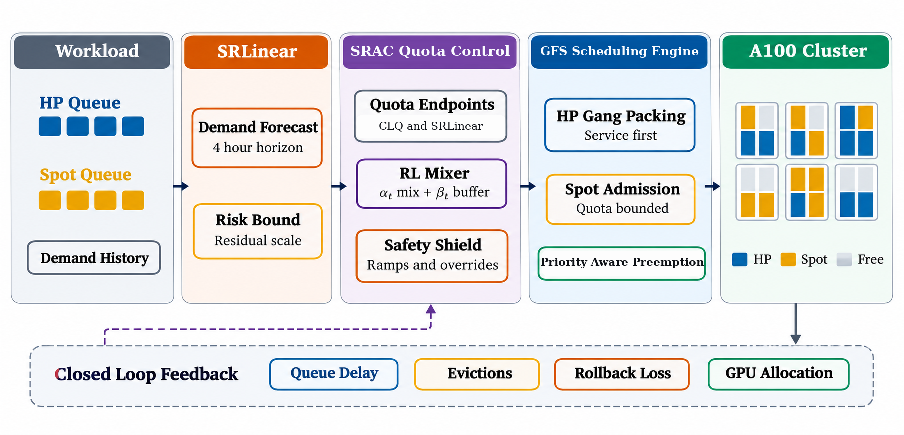
\includegraphics[width=\textwidth]{fig02_srac_system_architecture.pdf}
\caption{Forecast guided quota control and GFS scheduling framework.}
\label{fig:system}
\end{figure*}

\section{Related Work}
GFS is the closest system to this work. It predicts organization demand, computes a dynamic Spot quota and applies preemption aware scheduling~\cite{gfs}. Its control path remains deterministic after forecasting. Forecast uncertainty is not passed to a learned policy with cumulative rollback and service budgets. HiveD instead isolates tenant guarantees through virtual private clusters and lets low priority jobs use idle capacity~\cite{hived}. DeepShare coordinates quota borrowing, queue ordering, preemption and GPU sharing through a tenant assurance signal~\cite{deepshare}. These systems provide strong resource sharing controls. They do not adapt a forecast guided Spot quota from current uncertainty and rollback risk.

Placement methods address a different source of inefficiency. Fragmentation Gradient Descent directs placement toward lower fractional GPU fragmentation~\cite{fgd}. DRR learns defragmentation placement with job rescheduling~\cite{drr}. RLTune learns job priorities before placement is solved across heterogeneous traces~\cite{rltune}. These methods act mainly through placement or relocation. The studied A100 pool uses whole GPUs and contains many equivalent placement choices. Quota control retains more authority because it changes how much Spot demand is admitted before future high priority arrivals.

The wider scheduler literature addresses unknown duration, topology, fairness, heterogeneity and elastic training. Tiresias uses attained service scheduling~\cite{tiresias}. Gandiva combines introspection with migration and time slicing~\cite{gandiva}. Themis uses auction based allocation for finish time fairness~\cite{themis}. Gavel models heterogeneous accelerator throughput~\cite{gavel}. Pollux adapts training and allocation through goodput~\cite{pollux}. Shockwave plans model adaptation under fairness goals~\cite{shockwave}. AntMan coordinates resource scaling and GPU sharing~\cite{antman}. Forecast uncertainty is not used as a bounded action for constrained preemptible quota control in these systems.

Forecasting methods provide another relevant foundation. NLinear and DLinear use simple linear projections for long horizon prediction~\cite{dlinear}. PatchTST models longer histories through temporal patches and channel independent attention~\cite{patchtst}. Mamba replaces attention with selective state space dynamics~\cite{mamba}. These general forecasters do not enforce equality between organization forecasts and the aggregate pool forecast required by quota allocation. GFS introduces OrgLinear for organization demand~\cite{gfs}. It does not include exact hierarchy reconciliation with a separate direct aggregate path. SRLinear addresses this gap through seasonal mixtures, small residual heads and exact reconciliation to a direct pool estimate.

SRAC builds on proximal policy optimization (PPO), generalized advantage estimation (GAE) and constrained policy learning~\cite{ppo,gae,cpo}. Existing learned GPU schedulers mainly control priority, placement or fragmentation~\cite{rltune,drr}. SRAC instead mixes a deterministic quota with a coherent forecast endpoint and deducts calibrated uncertainty under explicit operating budgets. Table~\ref{tab:gap} compares the closest method families. No reviewed method combines exact forecast coherence, online uncertainty actions, constrained recurrent quota learning and parity with a deterministic scheduler. This combination defines the research gap addressed here.

\begin{table*}[t]
\centering
\caption{Capability comparison for closely related GPU scheduling methods.}
\label{tab:gap}
\scriptsize
\setlength{\tabcolsep}{4.5pt}
\begin{tabular}{llllll}
\toprule
Method & Main decision & Demand forecast & Learned online control & Explicit risk budgets & Exact hierarchy coherence \\
\midrule
GFS~\cite{gfs} & Spot quota and preemption & OrgLinear & No & No & No \\
HiveD~\cite{hived} & Tenant isolation and scavenging & No & No & Hard sharing guarantee & No \\
FGD~\cite{fgd} & Fractional GPU placement & No & No & No & No \\
DRR~\cite{drr} & Placement and rescheduling & No & Yes & No & No \\
RLTune~\cite{rltune} & Priority and placement & Runtime features & Yes & No & No \\
DeepShare~\cite{deepshare} & Borrowing, preemption and sharing & Runtime prediction & No & Assurance signal & No \\
SRLinear with SRAC & Five minute Spot quota & SRLinear & Yes & Three cumulative costs & Yes \\
\bottomrule
\end{tabular}
\end{table*}

\section{Methodology}
\subsection{Problem formulation}
The cluster contains capacity $C$ and two job classes. High priority jobs have mandatory service. Spot jobs are admitted under quota $q_t$ and can be preempted. Every five minutes, the controller observes causal capacity, queue, forecast and risk state $s_t$, then selects $q_t$.

The primary throughput metric is useful Spot GPU hours $U$. Risk metrics are rollback lost GPU hours $L$, Spot queue GPU hours $Q_S$, high priority queue GPU hours $Q_H$, high priority gang violation rate $V_H$ and eviction count $E$. A method is feasible when $V_H \leq 2\%$. The control objective is to retain near ceiling $U$ while reducing destructive preemption and maintaining this service limit.

\subsection{SRLinear forecaster}
SRLinear is shown in Figure~\ref{fig:srlinear}. A 672 hour history from 28 organization demand series is received and four hourly horizons are predicted. Lags of 24, 48, 168, 336 and 672 hours are used by five causal anchors. The residual input is formed from recent means, slopes, a 48 hour residual history, hour and weekday features.

For organization $o$, horizon $h$ and anchor $k$, a convex gate forms the seasonal base
\begin{equation}
s_{t,h,o}=\sum_k g_{t,h,k}a_{t,h,o,k}, \qquad
g_{t,h}=\operatorname{softmax}(W_hx_t+b_h)
\end{equation}
An organization residual is added by a small linear head. Aggregate pool demand is predicted by a separate head. The sum of organization estimates is blended with the direct pool estimate by a learned scalar. If $z_{t,h,o}$ is the nonnegative organization estimate and $p_{t,h}$ is the final pool estimate, exact reconciliation is given by
\begin{equation}
\hat y_{t,h,o}=p_{t,h}\frac{z_{t,h,o}}{\sum_j z_{t,h,j}},
\qquad \sum_o \hat y_{t,h,o}=p_{t,h}
\end{equation}
Training is performed with the composite normalized loss
\begin{equation}
\mathcal L = L_{\mathrm{MAE}}+0.75L_{\mathrm{RMSE}}+0.25L_{\mathrm{tail}}
+0.20L_{\mathrm{peak}}+0.25L_{\mathrm{under}}
\end{equation}
Organization mean absolute error is assigned a weight of 0.15. Gate regularization is assigned a weight of $10^{-4}$. Peak thresholds and Gaussian residual scale are fitted only from causal training history.

\begin{figure*}[t]
\centering
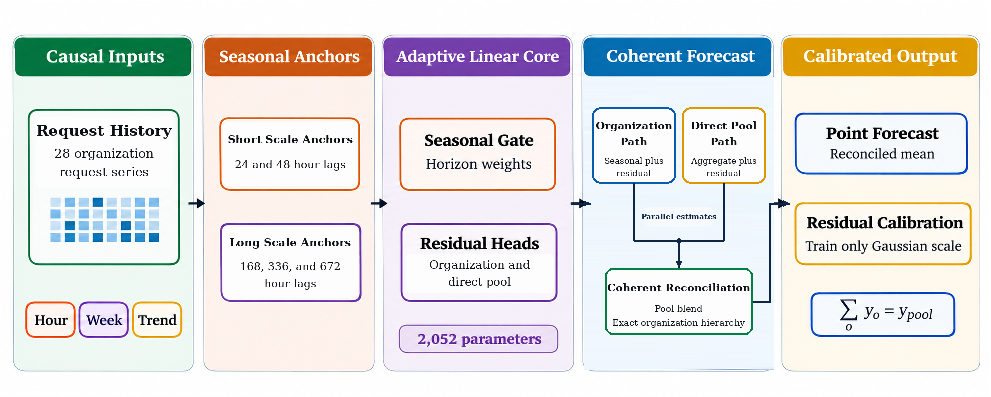
\includegraphics[width=\textwidth]{fig01_srlinear_architecture.pdf}
\caption{SRLinear causal forecasting architecture.}
\label{fig:srlinear}
\end{figure*}

\subsection{SRAC quota controller}
Thirty eight normalized features are received by SRAC. Capacity, queues, the two quota endpoints, forecast uncertainty, prior actions, recent costs, remaining budgets and calendar phase are represented. Two actor outputs, one reward value and three cost values are produced by a linear encoder and a 64 unit gated recurrent unit. A bounded Gaussian policy is used by the actor.

The SRLinear quota $q_t^{SR}$ is mixed with the CLQ endpoint $q_t^{CLQ}$ by the first action $\alpha_t\in[0,1]$. SRLinear uncertainty $\sigma_t$ is deducted by the second action $\beta_t\in[0,1]$:
\begin{equation}
q_t=\operatorname{clip}\left(\alpha_t q_t^{SR}+(1-\alpha_t)q_t^{CLQ}
-\beta_t\sigma_t,0,C\right)
\label{eq:srac}
\end{equation}
CLQ is exactly reproduced by the zero action. Changes in $\alpha_t$ and $\beta_t$ are limited by the safety shield to 0.25 per decision. When a high priority queue is active or a risk budget is exhausted, $\alpha_t=0$ and $\beta_t=1$ are enforced.

Recurrent PPO with GAE is used for the policy. The discount is 0.99, the GAE factor is 0.95, the rollout length is 256 and four PPO epochs are applied to each rollout. Normalized useful Spot work is added to the reward. Weighted Spot queue, rollback loss, high priority queue exposure and action variation are subtracted. High priority violations, rollback loss and high priority queue exposure are tracked by separate Lagrange multipliers. The learning loop is shown in Figure~\ref{fig:sracagent}.

\begin{figure*}[t]
\centering
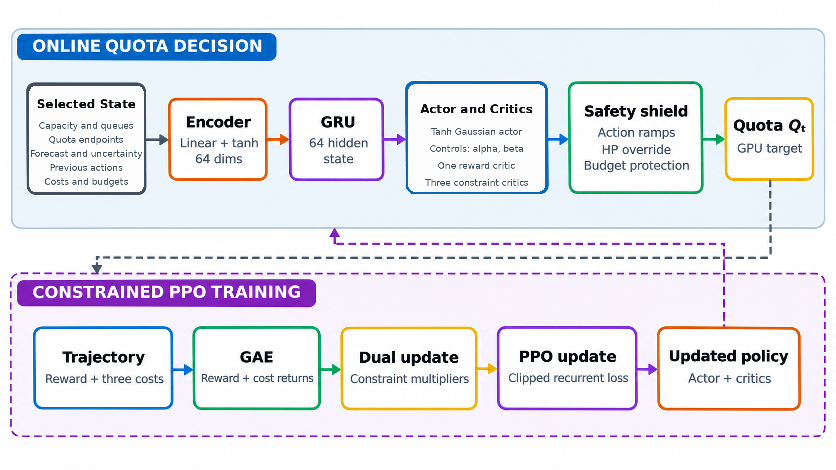
\includegraphics[width=0.98\textwidth]{fig03_srac_rl_agent_architecture.pdf}
\caption{SRAC recurrent actor critic and constrained PPO training loop.}
\label{fig:sracagent}
\end{figure*}

\section{Experimental Setup}
High priority and Spot jobs across six GPU types are contained in the Alibaba Spot GPU trace~\cite{alibabatrace}. A100 SXM4 80GB nodes are selected for the primary benchmark, which contains 3,456 GPUs. March and April 2024 are used for warmup. May and June are used for training and forecast development. The period from July 2 through July 31 is used for 720 validation hours and 8,640 five minute decisions. Adjacent splits are separated by a one day embargo. August remains locked and is not used in this paper.

The July workload contains 21,249 high priority arrivals and 7,831 Spot arrivals. Sixty one daily origins, a 672 hour lookback and a four hour horizon are used for forecasting. Three seeds derived from master seed 17 are used for stochastic methods. One run is used for deterministic methods after parity and determinism checks.

All methods use one event simulation environment with common chronological events, quota actions, queue accounting, preemption loss and completion credit. The same trace split, warmup state and metric definitions are applied to every comparison. Forecast and policy fitting use only training history. Independent simulation runs use separate CPU processes. Learned tensor operations use CUDA.

Forecast baselines are Seasonal Naive, OrgLinear from GFS, NLinear, DLinear, Temporal Mamba and PatchTST. Scheduling baselines include Native GFS, quota rules, CLQ, YARN-CS~\cite{yarn}, Chronus~\cite{chronus}, Lyra~\cite{lyra} and FGD~\cite{fgd}. The last four reproduce their stated queue, lease, cost or fragmentation mechanism in the common environment. They are not full reproductions of the external systems. RL baselines share the same constrained recurrent PPO protocol. Stochastic results are reported as mean and standard deviation across three seeds.

\section{Results}
\subsection{Forecast accuracy and cost}
Forecasting accuracy and cost are compared in Table~\ref{tab:forecast} and Figure~\ref{fig:forecast}. The lowest mean absolute error, 154.964, is obtained by SRLinear. Mean absolute error is reduced relative to PatchTST by 5.27 percent, Temporal Mamba by 7.30 percent, DLinear by 8.60 percent and OrgLinear by 35.79 percent. A 0.65 percent lower root mean square error is retained by PatchTST. SRLinear contains 2,052 parameters and requires 10.372 thousand multiply accumulate operations. A runtime of 60.8 seconds is measured, which is 19.39 times faster than PatchTST and 70.73 times faster than OrgLinear.

\begin{table*}[t]
\centering
\caption{Forecast accuracy and computational cost over 61 rolling origins.}
\label{tab:forecast}
\scriptsize
\setlength{\tabcolsep}{3.3pt}
\begin{tabular}{lrrrrrl}
\toprule
Model & MAE $\downarrow$ & RMSE $\downarrow$ & Parameters $\downarrow$ & MACs $\downarrow$ & FLOPs $\downarrow$ & Runtime $\downarrow$ and device \\
\midrule
Seasonal Naive & 265.109 & 335.852 & 0 & 0 & 0 & 3.1 s, CPU \\
OrgLinear~\cite{gfs} & $241.357\pm20.229$ & $342.984\pm36.747$ & 10,004 & 274.848K & 549.696K & 71.67 min, CPU \\
NLinear~\cite{dlinear} & $187.220\pm2.509$ & $231.802\pm1.681$ & 2,692 & 75.264K & 150.528K & 1.56 min, CPU \\
DLinear~\cite{dlinear} & $169.548\pm3.974$ & $203.589\pm4.197$ & 5,384 & 150.528K & 301.056K & 2.55 min, CUDA \\
Temporal Mamba~\cite{mamba} & $167.161\pm1.710$ & $201.023\pm2.081$ & 12,900 & 8.555M & 17.110M & 23.42 min, CUDA \\
PatchTST~\cite{patchtst} & $163.593\pm0.611$ & $197.316\pm0.457$ & 94,724 & 204.661M & 409.321M & 19.65 min, CUDA \\
SRLinear & $154.964\pm0.130$ & $198.602\pm0.255$ & 2,052 & 10.372K & 20.744K & 60.8 s, CUDA \\
\bottomrule
\end{tabular}
\end{table*}

\begin{figure}[t]
\centering
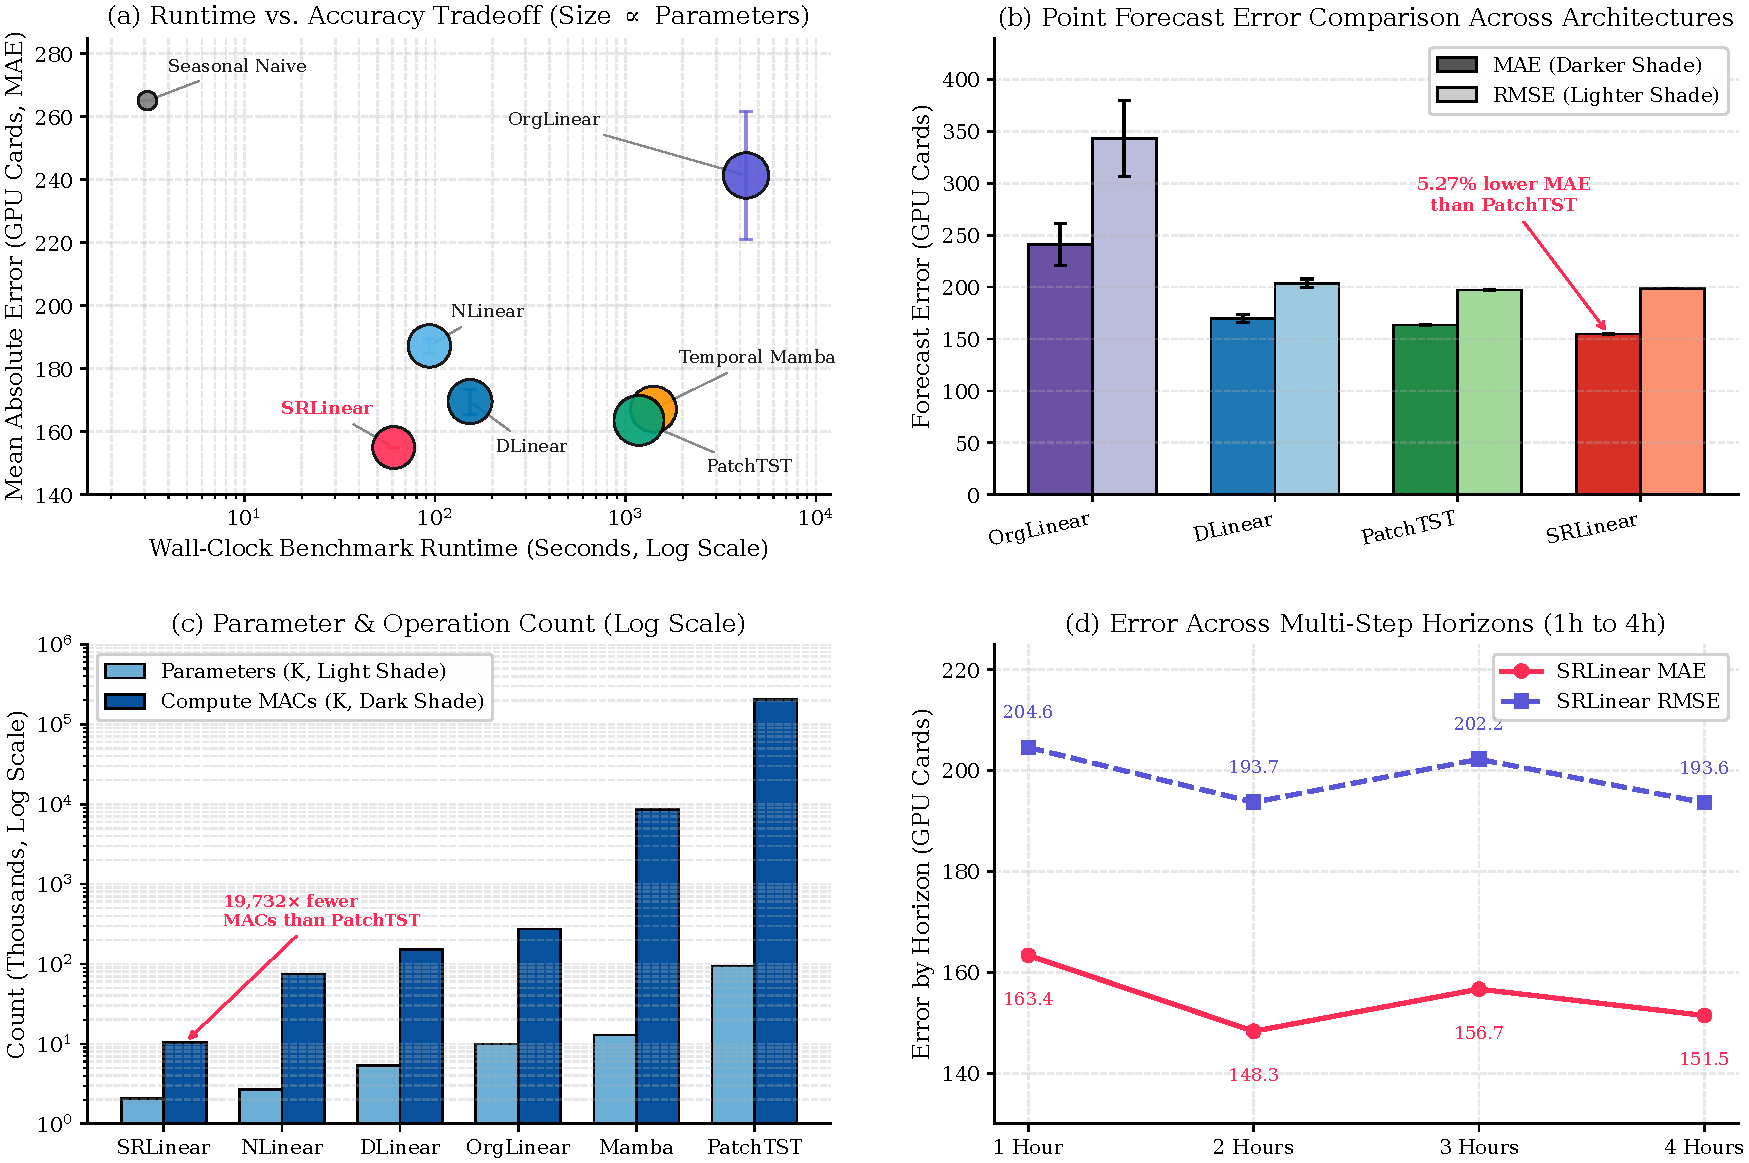
\includegraphics[width=\columnwidth]{fig04_forecast_benchmark_efficiency.pdf}
\caption{Forecast accuracy, runtime, model cost and horizon error.}
\label{fig:forecast}
\end{figure}

Figure~\ref{fig:forecast}(d) shows SRLinear error by horizon. Mean absolute error remains between 148.335 and 163.377. Bias reaches about $-19.5$ GPUs at the three and four hour horizons. This error pattern motivates the uncertainty deduction in SRAC instead of direct use of the point forecast.

\subsection{Deterministic scheduling}
Scheduling methods are compared in Table~\ref{tab:scheduling} and Figure~\ref{fig:scheduling}. SRGFS denotes GFS with OrgLinear replaced by SRLinear. SRMix denotes the deterministic SRLinear contextual mixture controller. A total of 96,146.494 useful Spot GPU hours is produced by Native GFS. With SRLinear, 96,392.645 hours are reached by SRGFS, which gives a 0.256 percent gain. The Spot queue is reduced from 193,469.732 to 27,812.635 GPU hours and the high priority violation rate is reduced from 1.448 to 0.483 percent. These changes correspond to an 85.6 percent queue reduction and a 66.7 percent violation reduction. Higher rollback loss and more evictions are incurred.

CLQ reaches the largest deterministic useful work at 96,408.612 hours and the lowest high priority violation rate at 0.214 percent. SRMix retains 96,395.791 useful hours. Relative to SRGFS, it reduces rollback loss by 31.9 percent and evictions by 24.8 percent. All proposed variants satisfy the service limit.

\begin{table*}[t]
\centering
\caption{Non RL scheduling results on July validation.}
\label{tab:scheduling}
\scriptsize
\setlength{\tabcolsep}{2.2pt}
\resizebox{\textwidth}{!}{%
\begin{tabular}{lrrrrrrr}
\toprule
Method & Useful Spot GPU h $\uparrow$ & Lost GPU h $\downarrow$ & Spot queue GPU h $\downarrow$ & HP queue GPU h $\downarrow$ & HP violation $\downarrow$ & Evictions $\downarrow$ \\
\midrule
Native GFS~\cite{gfs} & 96,146.494 & 329.007 & 193,469.732 & 9,342.260 & 1.448\% & 128 \\
FCFS Admission & 96,391.645 & 1,292.174 & 143,439.405 & 7,467.322 & 1.340\% & 148 \\
GFS Causal SEPT~\cite{gfs} & 96,248.768 & 422.147 & 174,605.279 & 9,808.964 & 1.662\% & 114 \\
Fixed Residual Quota & 96,242.809 & 319.434 & 250,029.435 & 7,287.682 & 1.555\% & 86 \\
Diurnal Quota Control & 96,330.669 & 609.250 & 84,168.283 & 4,501.687 & 0.751\% & 134 \\
Online Quantile Control & 93,437.811 & 395.676 & 218,313.164 & 4,435.596 & 0.751\% & 105 \\
Headroom Reserve Control & 96,389.645 & 604.595 & 170,447.132 & 9,746.598 & 1.609\% & 244 \\
CLQ & 96,408.612 & 640.240 & 39,883.449 & 3,001.269 & 0.214\% & 245 \\
YARN-CS~\cite{yarn} & 96,162.393 & 33,810.634 & 149,163.224 & 789.551 & 0.214\% & 12,404 \\
Chronus~\cite{chronus} & 96,216.438 & 0.000 & 96,175.589 & 16,033.177 & 0.322\% & 0 \\
Lyra~\cite{lyra} & 96,375.874 & 946.913 & 106,065.391 & 14,216.720 & 2.198\% & 123 \\
FGD~\cite{fgd} & 96,125.162 & 43,354.449 & 180,870.467 & 845.282 & 0.214\% & 12,187 \\
SRGFS & $96,392.645\pm0.000$ & $1,195.832\pm49.747$ & $27,812.635\pm476.561$ & $3,816.404\pm1,195.746$ & $0.483\pm0.186$\% & $314.0\pm5.2$ \\
SRMix & $96,395.791\pm4.839$ & $814.693\pm309.730$ & $64,216.750\pm12,320.898$ & $5,433.191\pm2,797.660$ & $0.858\pm0.597$\% & $236.0\pm6.6$ \\
\bottomrule
\end{tabular}}
\end{table*}

\begin{figure}[t]
\centering
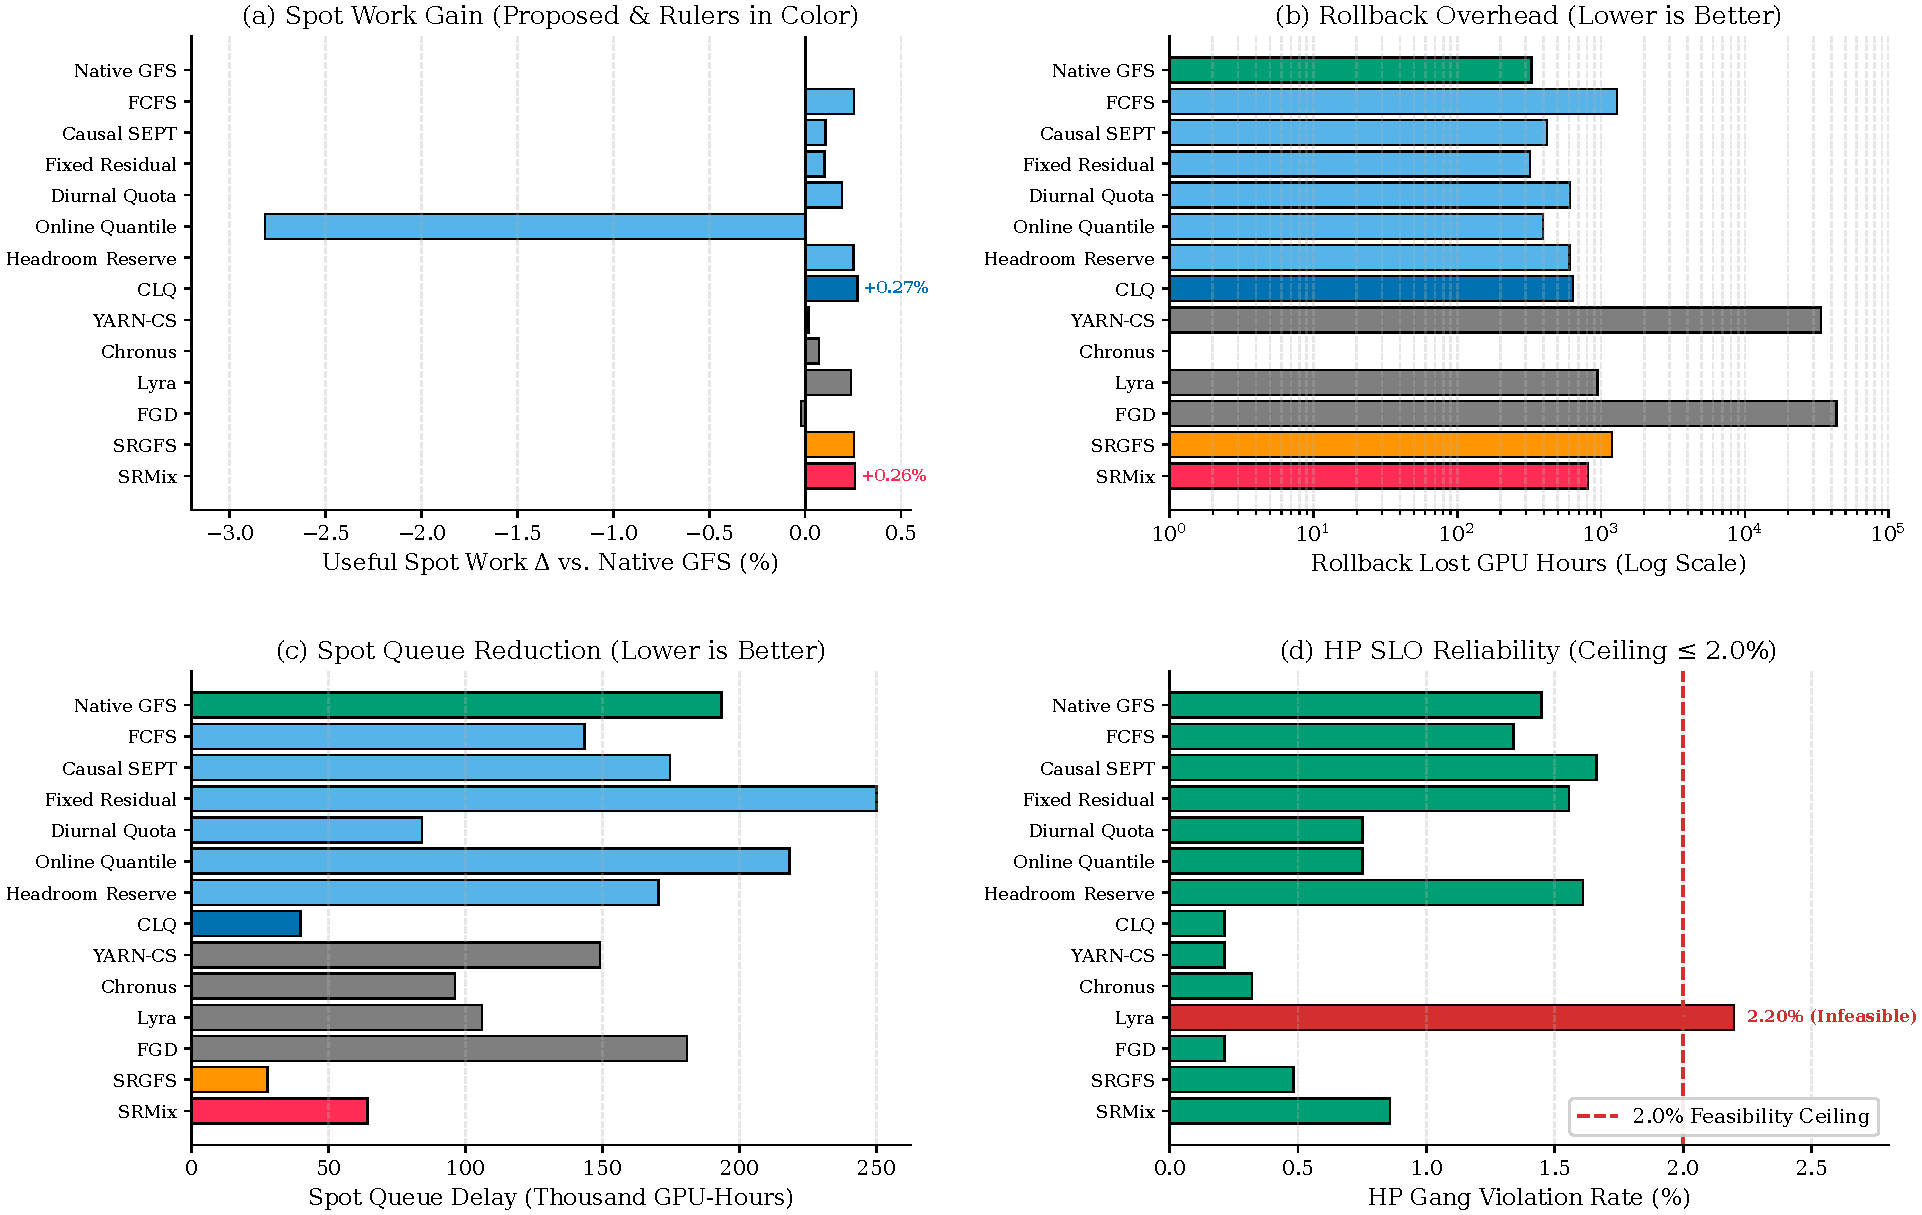
\includegraphics[width=\columnwidth]{fig05_non_rl_scheduling_comparison.pdf}
\caption{Non RL scheduling throughput, rollback, queue and service metrics.}
\label{fig:scheduling}
\end{figure}

\subsection{Forecast guided reinforcement learning}
SRAC is compared with deterministic rulers and other quota RL variants in Table~\ref{tab:rl} and Figure~\ref{fig:rl}. CLQ-PPO applies recurrent PPO to CLQ, SRU-PPO uses the SRLinear utility objective and SRQ-PPO controls the SRLinear quota endpoint. SRAC obtains the lowest rollback loss and eviction count among the active RL methods. Relative to CLQ, it retains 99.9507 percent of useful work, reduces rollback loss from 640.240 to 621.251 GPU hours and reduces evictions from 245 to 233.3. The high priority violation rate increases from 0.2145 to 1.5550 percent. It remains below the fixed 2 percent constraint.

The comparison also indicates why useful work alone is not a sufficient RL reward. SRU-PPO reaches 96,398.457 useful hours. It also incurs 1,898.094 lost GPU hours and 395.3 evictions. SRAC reaches a lower loss region while preserving nearly all useful work. Figure~\ref{fig:rl} shows this risk and throughput frontier.

\begin{table*}[t]
\centering
\caption{Forecast guided reinforcement learning results on July validation.}
\label{tab:rl}
\scriptsize
\setlength{\tabcolsep}{2.7pt}
\resizebox{\textwidth}{!}{%
\begin{tabular}{lrrrrrr}
\toprule
Method & Useful Spot GPU h $\uparrow$ & Lost GPU h $\downarrow$ & Spot queue GPU h $\downarrow$ & HP queue GPU h $\downarrow$ & HP violation $\downarrow$ & Evictions $\downarrow$ \\
\midrule
CLQ & 96,408.612 & 640.240 & 39,883.449 & 3,001.269 & 0.2145\% & 245 \\
SRGFS & $96,392.645\pm0.000$ & $1,195.832\pm49.747$ & $27,812.635\pm476.561$ & $3,816.404\pm1,195.746$ & $0.4826\pm0.1857$\% & $314.0\pm5.2$ \\
CLQ-PPO & $96,384.645\pm0.000$ & $723.666\pm0.000$ & $41,098.610\pm0.000$ & $10,925.018\pm0.000$ & $1.8231\pm0.0000$\% & $254.0\pm0.0$ \\
SRU-PPO & $96,398.457\pm5.033$ & $1,898.094\pm638.458$ & $58,789.675\pm29,816.994$ & $5,932.021\pm1,236.295$ & $1.0009\pm0.4024$\% & $395.3\pm73.2$ \\
SRQ-PPO & $96,261.064\pm123.656$ & $976.155\pm378.156$ & $143,054.431\pm72,698.915$ & $8,087.384\pm1,790.111$ & $1.3762\pm0.3650$\% & $262.7\pm27.6$ \\
SRAC & $96,361.058\pm4.592$ & $621.251\pm80.371$ & $44,637.025\pm13,417.365$ & $8,426.727\pm1,134.190$ & $1.5550\pm0.1857$\% & $233.3\pm20.6$ \\
\bottomrule
\end{tabular}}
\end{table*}

\begin{figure}[t]
\centering
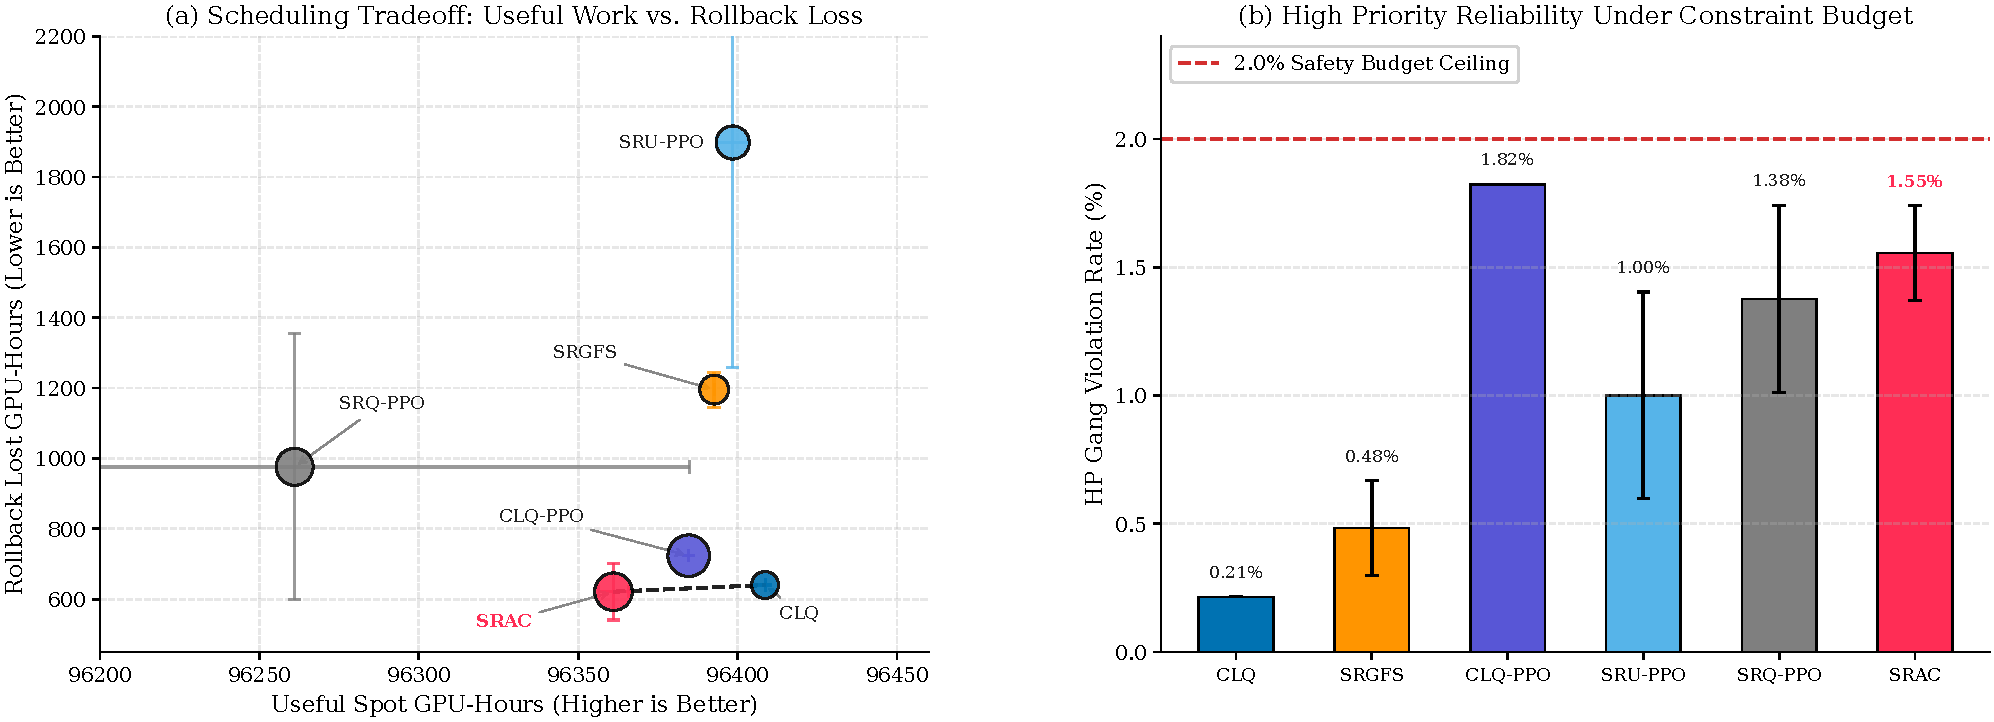
\includegraphics[width=\columnwidth]{fig06_rl_comparison_tradeoffs.pdf}
\caption{RL throughput, rollback and high priority service tradeoffs.}
\label{fig:rl}
\end{figure}

\subsection{Mechanism ablation}
Seasonal Residual Quantile Guard (SRQGuard) is isolated by component in Table~\ref{tab:ablation}. The SRLinear quantile quota reaches 96,393.200 useful hours and reduces the Spot queue by 88.8 percent relative to Native GFS. Adding causal priority changes the queue and rollback balance. The guarded quota reaches similar useful work and a smaller Spot queue. It also produces more evictions. Replacing SRLinear with OrgLinear lowers useful work to 96,257.874 hours and increases the Spot queue to 37,883.630 GPU hours. Figure~\ref{fig:ablation} compares throughput, queue, rollback and eviction metrics.

\begin{table*}[t]
\centering
\caption{SRQGuard mechanism ablations on July validation.}
\label{tab:ablation}
\scriptsize
\setlength{\tabcolsep}{3.0pt}
\resizebox{\textwidth}{!}{%
\begin{tabular}{llrrrrrr}
\toprule
Variant & Change & Useful Spot GPU h $\uparrow$ & Lost GPU h $\downarrow$ & Spot queue GPU h $\downarrow$ & HP queue GPU h $\downarrow$ & HP violation $\downarrow$ & Evictions $\downarrow$ \\
\midrule
Native GFS~\cite{gfs} & Reference & 96,146.494 & 329.007 & 193,469.732 & 9,342.260 & 1.448\% & 128 \\
SRQGuard Quota & SRLinear quantile quota & $96,393.200\pm7.900$ & $2,125.834\pm508.569$ & $21,694.336\pm259.304$ & $6,917.487\pm2,301.584$ & $1.019\pm0.429$\% & $340.3\pm50.5$ \\
SRQGuard Priority & Add causal priority & $96,387.943\pm12.413$ & $1,795.432\pm453.363$ & $26,622.686\pm218.229$ & $7,811.610\pm2,173.718$ & $1.215\pm0.573$\% & $392.7\pm25.1$ \\
SRQGuard Full & Add guarded quota & $96,393.124\pm0.414$ & $1,827.164\pm528.358$ & $17,873.111\pm1,133.256$ & $7,258.418\pm2,918.091$ & $1.126\pm0.609$\% & $486.7\pm40.7$ \\
SRQGuard No Aging & Remove aging & $96,395.551\pm5.033$ & $2,148.301\pm324.354$ & $14,734.131\pm86.890$ & $7,755.526\pm256.762$ & $1.394\pm0.186$\% & $340.3\pm24.8$ \\
OrgQGuard~\cite{gfs} & Replace SRLinear & 96,257.874 & 1,035.536 & 37,883.630 & 9,121.756 & 1.448\% & 233 \\
\bottomrule
\end{tabular}}
\end{table*}

\noindent\begin{minipage}{\columnwidth}
\subsection{Controller behavior}
Figure~\ref{fig:dynamics} shows an executed SRAC validation ledger. The 72 hour interval is selected by maximum high priority queue exposure rather than favorable outcome. SRLinear and CLQ differ by several hundred GPUs in parts of this window. SRAC follows the protected endpoint after the risk shield is activated. The shield dominates the executed action and the uncertainty coefficient remains at its protective limit. The event raster aligns rollback loss and high priority violations with the same interval. Therefore, SRAC reduces rollback loss and evictions by using more of the allowed high priority service budget.
\end{minipage}

\begin{figure}[t]
\centering
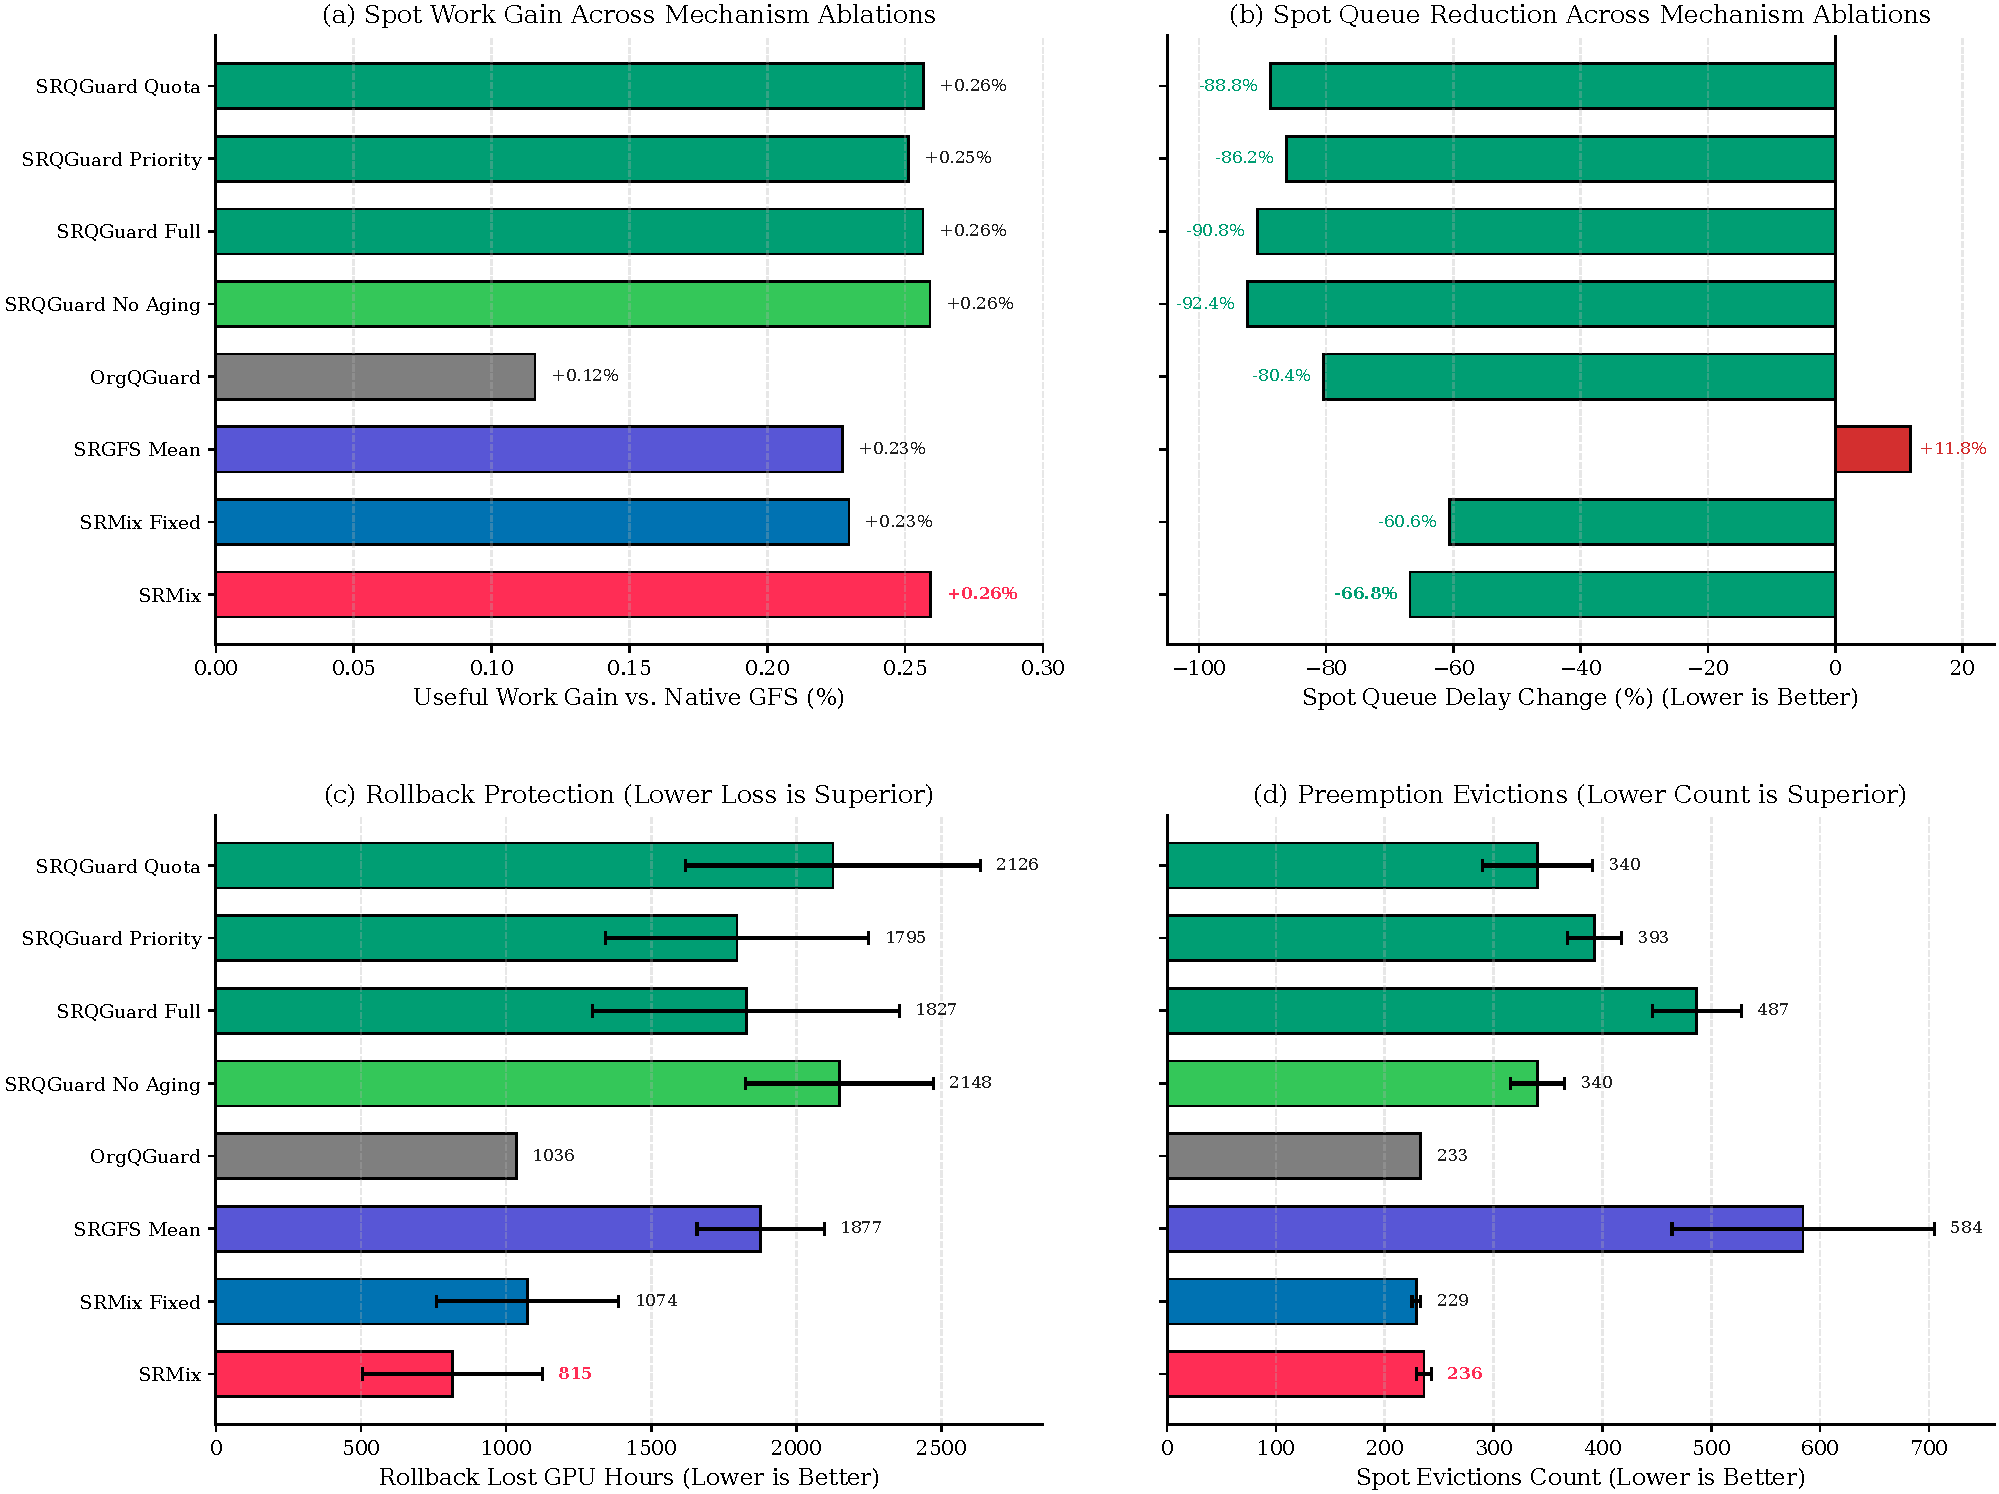
\includegraphics[width=\columnwidth]{fig07_mechanism_ablations.pdf}
\caption{Throughput, queue, rollback and eviction results for mechanism ablations.}
\label{fig:ablation}
\end{figure}

\begin{figure}[!t]
\centering
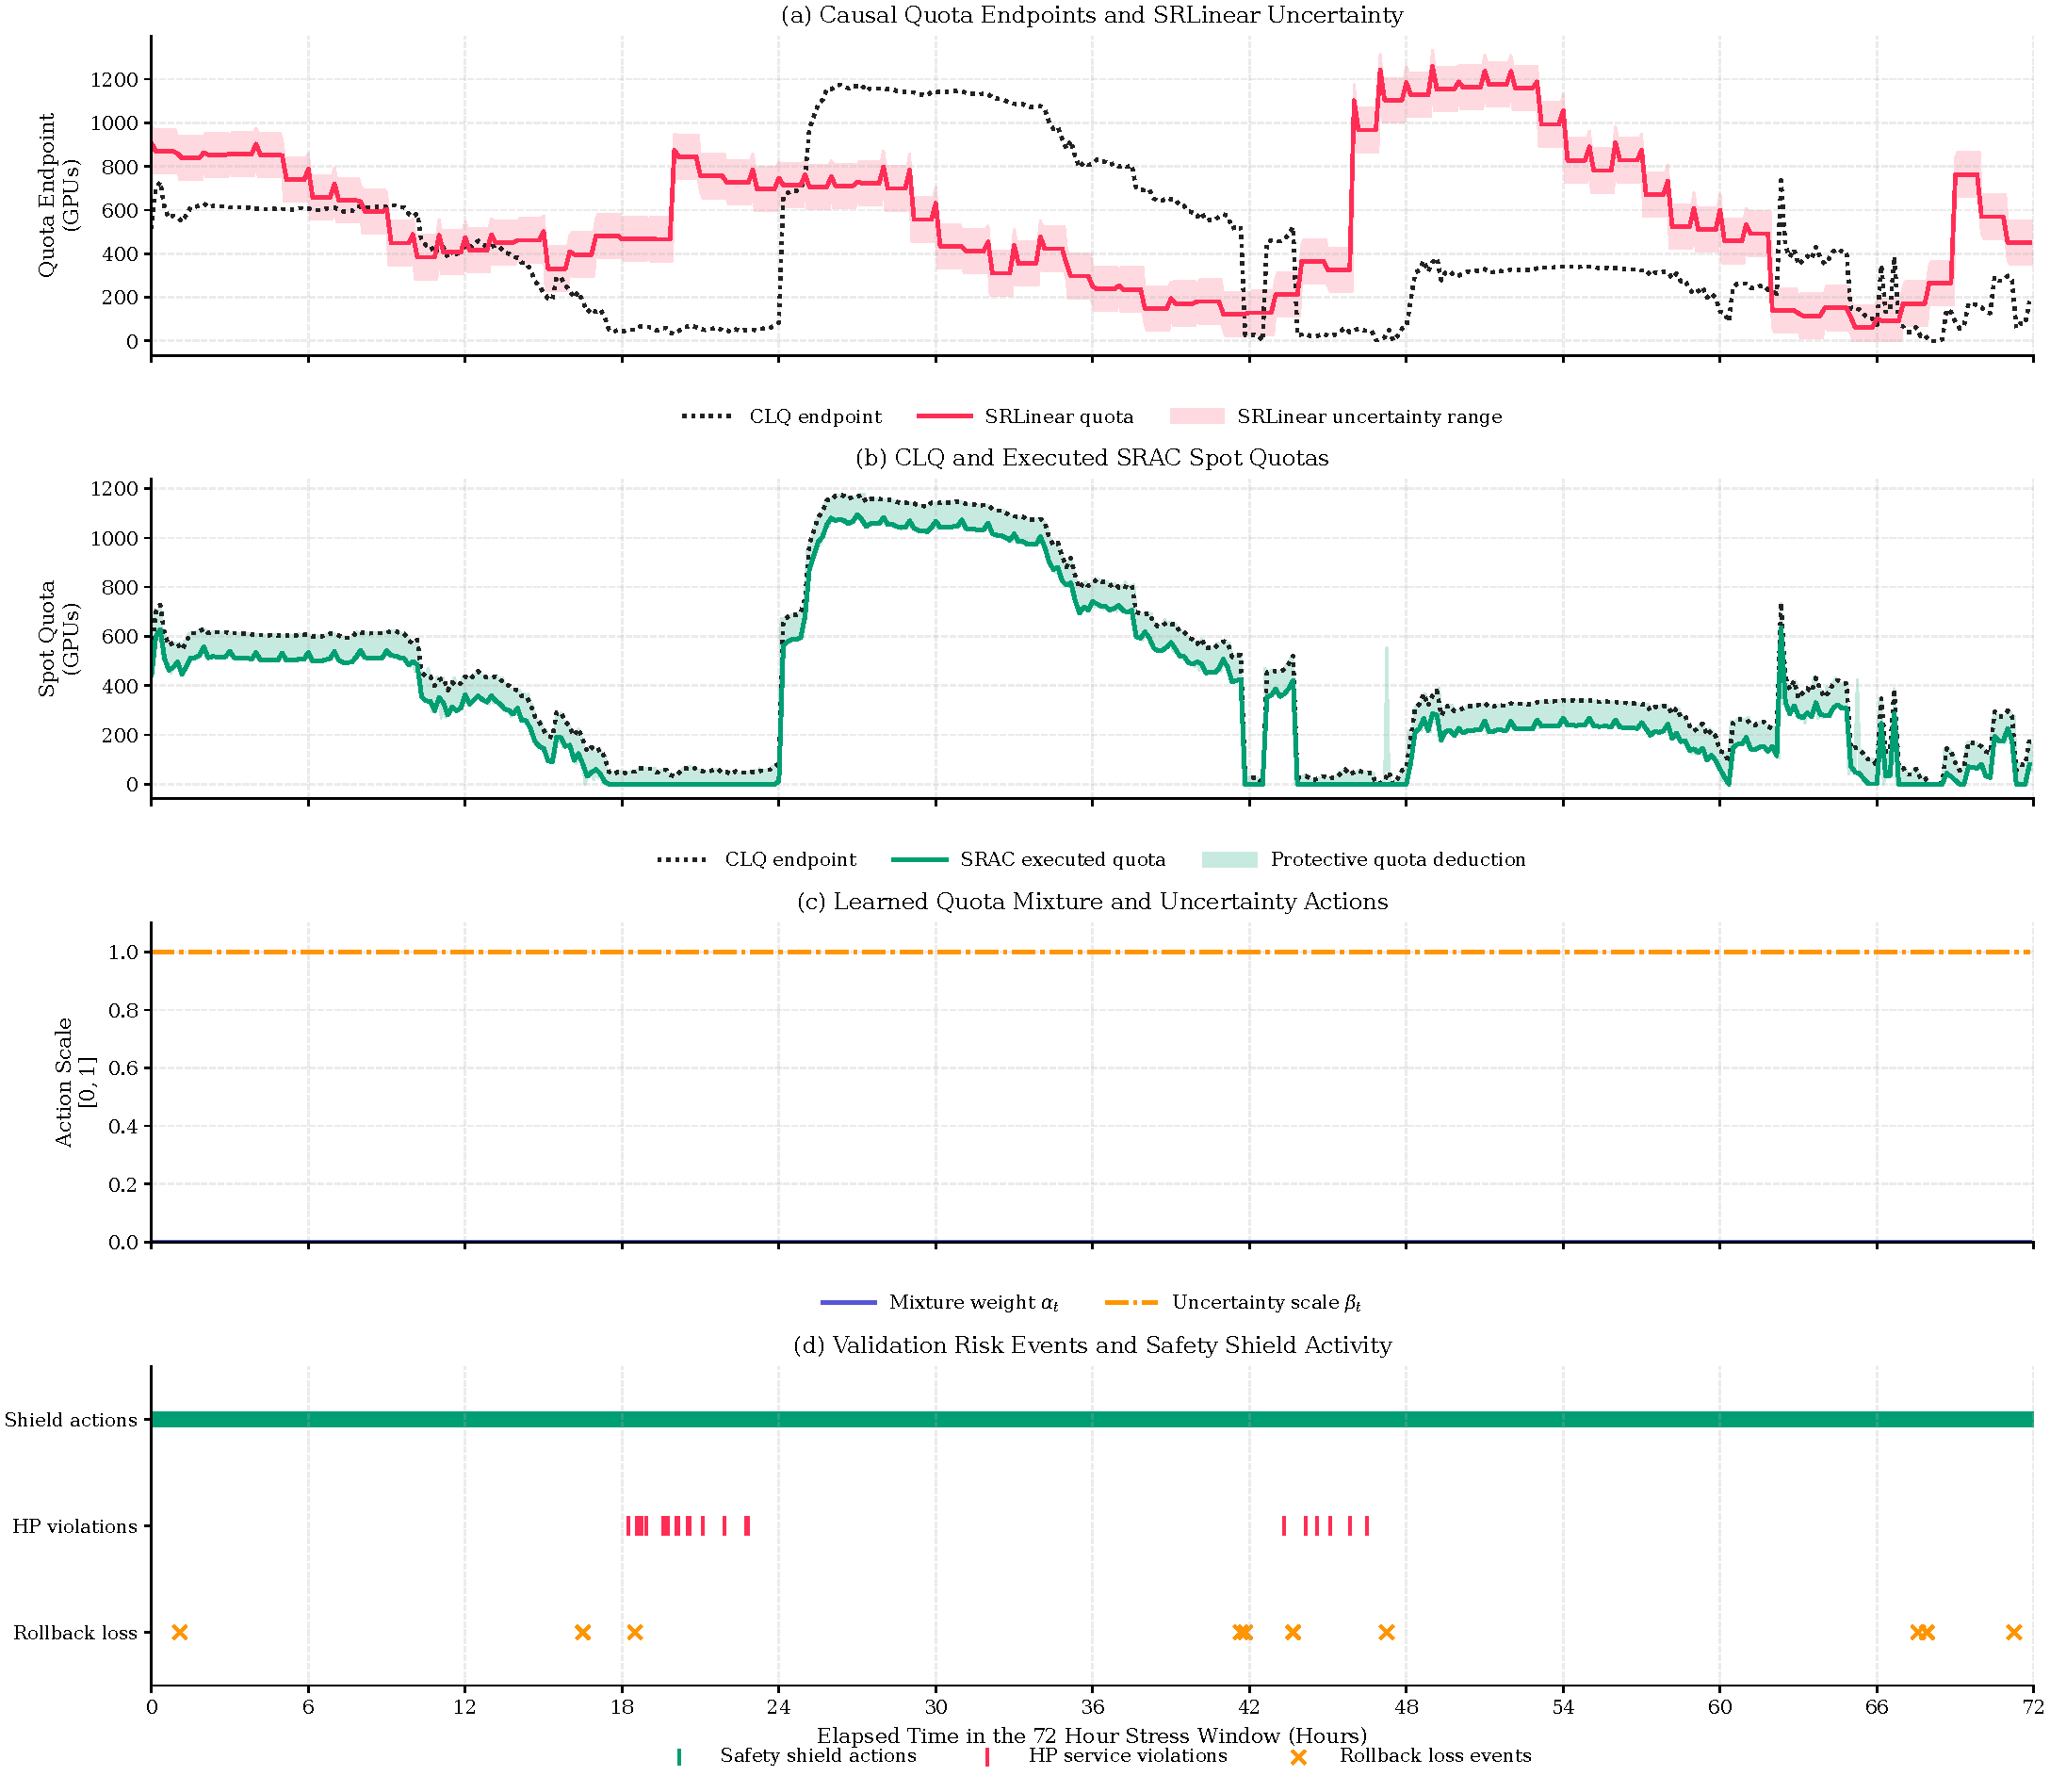
\includegraphics[width=\columnwidth]{fig08_srac_policy_dynamics.pdf}
\caption{SRAC quota endpoints, executed actions and risk events in the maximum high priority queue exposure window.}
\label{fig:dynamics}
\end{figure}

\section{Discussion}
The clearest gain is provided by SRLinear. Its seasonal structure matches the trace and its aggregate path avoids error accumulation from independent organization forecasts. Exact reconciliation keeps organization forecasts usable by GFS quota logic. This design explains why a small model can reduce mean absolute error and compute relative to the tested neural baselines.

Scheduling gains are smaller because useful Spot work is near the natural trace ceiling. The relevant operating point is therefore multi objective. SRGFS exposes more useful capacity than Native GFS and reduces queues and service violations. CLQ remains the strongest deterministic ruler for useful work. SRAC does not exceed that value. It instead reduces rollback and eviction cost while satisfying the high priority constraint. The result is a risk tradeoff rather than uniform dominance.

Three limitations define the evidence. First, all scheduling values are July validation results. August remains locked. Second, the benchmark uses one homogeneous A100 pool. Different results may be obtained under heterogeneous GPUs or fractional sharing. Third, the shield dominates behavior under the highest pressure. This improves operational safety. It also limits attribution of the final action to the learned actor. Future work should evaluate the locked test and study stronger risk features and more direct constraint aware policy updates.

\section{Conclusion}
This paper presented SRLinear and SRAC for forecast guided quota control in preemptible GPU clusters. SRLinear combines causal seasonality, residual prediction and exact hierarchy reconciliation in a small model. SRGFS increases useful Spot work and reduces queue and service violations relative to Native GFS. SRAC uses constrained recurrent PPO to reduce rollback loss and evictions relative to CLQ while preserving near ceiling useful work. The evidence supports coherent forecasting and risk aware sequential control as complementary scheduling components. Evaluation on one homogeneous GPU type remains the main limitation.

\begin{thebibliography}{23}

\bibitem{gfs}
J. Duan et al., \href{https://doi.org/10.1145/3760250.3762231}{``GFS: A preemption-aware scheduling framework for GPU clusters with predictive Spot instance management,''} in \emph{Proc. 31st ACM Int. Conf. Architectural Support for Programming Languages and Operating Systems}, vol. 1, 2026, pp. 117--131, doi: 10.1145/3760250.3762231.

\bibitem{hived}
H. Zhao et al., \href{https://www.usenix.org/conference/osdi20/presentation/zhao-hanyu}{``HiveD: Sharing a GPU cluster for deep learning with guarantees,''} in \emph{Proc. 14th USENIX Symp. Operating Systems Design and Implementation}, 2020, pp. 515--532.

\bibitem{fgd}
Q. Weng, L. Yang, Y. Yu, W. Wang, X. Tang, G. Yang and L. Zhang, \href{https://www.usenix.org/conference/atc23/presentation/weng}{``Beware of fragmentation: Scheduling GPU-sharing workloads with fragmentation gradient descent,''} in \emph{Proc. USENIX Annual Technical Conf.}, 2023, pp. 995--1008.

\bibitem{drr}
Q. Wu, P. Chen and Y. Wang, \href{https://doi.org/10.1145/3772052.3772242}{``Defragmentation scheduling with deep reinforcement learning in shared GPU clusters,''} in \emph{Proc. ACM Symp. Cloud Computing}, 2025, pp. 402--415, doi: 10.1145/3772052.3772242.

\bibitem{deepshare}
J. Wang et al., \href{https://doi.org/10.1109/CLUSTER68337.2026.00015}{``DeepShare: Assurance-driven deep learning job scheduling for multi-tenant clusters,''} in \emph{Proc. 2026 IEEE Int. Conf. Cluster Computing}, 2026, pp. 1--13, doi: 10.1109/CLUSTER68337.2026.00015.

\bibitem{rltune}
S. Dongare, R. I. S. Khan, H. Albahar, N. Zhao, D. M. Maita and A. R. Butt, \href{https://doi.org/10.1145/3772052.3772257}{``Hybrid learning and optimization-based dynamic scheduling for DL workloads on heterogeneous GPU clusters,''} in \emph{Proc. 2025 ACM Symp. Cloud Computing}, 2025, pp. 557--570, doi: 10.1145/3772052.3772257.

\bibitem{tiresias}
J. Gu et al., \href{https://www.usenix.org/conference/nsdi19/presentation/gu}{``Tiresias: A GPU cluster manager for distributed deep learning,''} in \emph{Proc. 16th USENIX Symp. Networked Systems Design and Implementation}, 2019, pp. 485--500.

\bibitem{gandiva}
W. Xiao et al., \href{https://www.usenix.org/conference/osdi18/presentation/xiao}{``Gandiva: Introspective cluster scheduling for deep learning,''} in \emph{Proc. 13th USENIX Symp. Operating Systems Design and Implementation}, 2018, pp. 595--610.

\bibitem{themis}
K. Mahajan et al., \href{https://www.usenix.org/conference/nsdi20/presentation/mahajan}{``Themis: Fair and efficient GPU cluster scheduling,''} in \emph{Proc. 17th USENIX Symp. Networked Systems Design and Implementation}, 2020, pp. 289--304.

\bibitem{gavel}
D. Narayanan, K. Santhanam, F. Kazhamiaka, A. Phanishayee and M. Zaharia, \href{https://www.usenix.org/conference/osdi20/presentation/narayanan-deepak}{``Heterogeneity-aware cluster scheduling policies for deep learning workloads,''} in \emph{Proc. 14th USENIX Symp. Operating Systems Design and Implementation}, 2020, pp. 481--498.

\bibitem{pollux}
A. Qiao et al., \href{https://www.usenix.org/conference/osdi21/presentation/qiao}{``Pollux: Co-adaptive cluster scheduling for goodput-optimized deep learning,''} in \emph{Proc. 15th USENIX Symp. Operating Systems Design and Implementation}, 2021, pp. 1--18.

\bibitem{shockwave}
P. Zheng, R. Pan, T. Khan, S. Venkataraman and A. Akella, \href{https://www.usenix.org/conference/nsdi23/presentation/zheng}{``Shockwave: Fair and efficient cluster scheduling for dynamic adaptation in machine learning,''} in \emph{Proc. 20th USENIX Symp. Networked Systems Design and Implementation}, 2023, pp. 703--723.

\bibitem{antman}
W. Xiao et al., \href{https://www.usenix.org/conference/osdi20/presentation/xiao}{``AntMan: Dynamic scaling on GPU clusters for deep learning,''} in \emph{Proc. 14th USENIX Symp. Operating Systems Design and Implementation}, 2020, pp. 533--548.

\bibitem{dlinear}
A. Zeng, M. Chen, L. Zhang and Q. Xu, \href{https://doi.org/10.1609/aaai.v37i9.26317}{``Are transformers effective for time series forecasting?''} in \emph{Proc. AAAI Conf. Artificial Intelligence}, vol. 37, no. 9, 2023, pp. 11121--11128, doi: 10.1609/aaai.v37i9.26317.

\bibitem{patchtst}
Y. Nie, N. H. Nguyen, P. Sinthong and J. Kalagnanam, \href{https://openreview.net/forum?id=Jbdc0vTOcol}{``A time series is worth 64 words: Long-term forecasting with transformers,''} in \emph{Proc. Int. Conf. Learning Representations}, 2023.

\bibitem{mamba}
A. Gu and T. Dao, \href{https://openreview.net/forum?id=tEYskw1VY2}{``Mamba: Linear-time sequence modeling with selective state spaces,''} in \emph{Proc. Conf. Language Modeling}, 2024.

\bibitem{ppo}
J. Schulman, F. Wolski, P. Dhariwal, A. Radford and O. Klimov, \href{https://arxiv.org/abs/1707.06347}{``Proximal policy optimization algorithms,''} \emph{arXiv preprint arXiv:1707.06347}, 2017.

\bibitem{gae}
J. Schulman, P. Moritz, S. Levine, M. I. Jordan and P. Abbeel, \href{https://arxiv.org/abs/1506.02438}{``High-dimensional continuous control using generalized advantage estimation,''} in \emph{Proc. 4th Int. Conf. Learning Representations}, 2016.

\bibitem{cpo}
J. Achiam, D. Held, A. Tamar and P. Abbeel, \href{https://proceedings.mlr.press/v70/achiam17a.html}{``Constrained policy optimization,''} in \emph{Proc. 34th Int. Conf. Machine Learning}, 2017, pp. 22--31.

\bibitem{alibabatrace}
Alibaba Group, \href{https://github.com/alibaba/clusterdata/tree/master/cluster-trace-v2026-spot-gpu}{``Traces for AI jobs leveraging Spot GPU resources,''} \emph{Alibaba Cluster Trace Program}, 2026. [Online]. Available: \url{https://github.com/alibaba/clusterdata/tree/master/cluster-trace-v2026-spot-gpu}.

\bibitem{yarn}
V. K. Vavilapalli et al., \href{https://doi.org/10.1145/2523616.2523633}{``Apache Hadoop YARN: Yet another resource negotiator,''} in \emph{Proc. 4th ACM Symp. Cloud Computing}, 2013, pp. 1--16, doi: 10.1145/2523616.2523633.

\bibitem{chronus}
W. Gao, Z. Ye, P. Sun, Y. Wen and T. Zhang, \href{https://doi.org/10.1145/3472883.3486978}{``Chronus: A novel deadline-aware scheduler for deep learning training jobs,''} in \emph{Proc. 2021 ACM Symp. Cloud Computing}, 2021, pp. 609--623, doi: 10.1145/3472883.3486978.

\bibitem{lyra}
J. Li, H. Xu, Y. Zhu, Z. Liu, C. Guo and C. Wang, \href{https://doi.org/10.1145/3552326.3587445}{``Lyra: Elastic scheduling for deep learning clusters,''} in \emph{Proc. 18th European Conf. Computer Systems}, 2023, pp. 835--850, doi: 10.1145/3552326.3587445.

\end{thebibliography}

\end{document}
